%% LyX 2.3.4.2 created this file.  For more info, see http://www.lyx.org/.
%% Do not edit unless you really know what you are doing.
\documentclass[english,dvipsnames,aspectratio=169]{beamer}
\usepackage{mathptmx}
\usepackage{eulervm}
\usepackage[T1]{fontenc}
\usepackage[latin9]{inputenc}
\usepackage{babel}
\usepackage{amstext}
\usepackage{amssymb}
\usepackage{graphicx}
\usepackage{ifthen}
\usepackage{xcolor}
\usepackage{xspace}
\usepackage{tikz}
\usetikzlibrary{tikzmark}
\usetikzlibrary{calc}
\usepackage{pgfplots}
%\pgfplotsset{compat=1.17}
\usepackage{booktabs}
\usepackage{xpatch}

\xpatchcmd{\itemize}
  {\def\makelabel}
  {\ifnum\@itemdepth=1\relax
     \setlength\itemsep{2ex}% separation for first level
   \else
     \ifnum\@itemdepth=2\relax
       \setlength\itemsep{1ex}% separation for second level
     \else
       \ifnum\@itemdepth=3\relax
         \setlength\itemsep{0.5ex}% separation for third level
   \fi\fi\fi\def\makelabel
  }
 {}
 {}

\ifx\hypersetup\undefined
  \AtBeginDocument{%
    \hypersetup{unicode=true,pdfusetitle,
 bookmarks=true,bookmarksnumbered=false,bookmarksopen=false,
 breaklinks=false,pdfborder={0 0 0},pdfborderstyle={},backref=false,colorlinks=true,
 allcolors=NYUPurple,urlcolor=LightPurple}
  }
\else
  \hypersetup{unicode=true,pdfusetitle,
 bookmarks=true,bookmarksnumbered=false,bookmarksopen=false,
 breaklinks=false,pdfborder={0 0 0},pdfborderstyle={},backref=false,colorlinks=true,
 allcolors=NYUPurple,urlcolor=LightPurple}
\fi

\makeatletter

%%%%%%%%%%%%%%%%%%%%%%%%%%%%%% LyX specific LaTeX commands.
%% Because html converters don't know tabularnewline
\providecommand{\tabularnewline}{\\}

%%%%%%%%%%%%%%%%%%%%%%%%%%%%%% Textclass specific LaTeX commands.
% this default might be overridden by plain title style
\newcommand\makebeamertitle{\frame{\maketitle}}%
% (ERT) argument for the TOC
\AtBeginDocument{%
  \let\origtableofcontents=\tableofcontents
  \def\tableofcontents{\@ifnextchar[{\origtableofcontents}{\gobbletableofcontents}}
  \def\gobbletableofcontents#1{\origtableofcontents}
}

%%%%%%%%%%%%%%%%%%%%%%%%%%%%%% User specified LaTeX commands.
\usetheme{CambridgeUS} 
\beamertemplatenavigationsymbolsempty


% Set Color ==============================
\definecolor{NYUPurple}{RGB}{87,6,140}
\definecolor{LightPurple}{RGB}{165,11,255}


\setbeamercolor{title}{fg=NYUPurple}
\setbeamercolor{frametitle}{fg=NYUPurple}

\setbeamercolor{background canvas}{fg=NYUPurple, bg=white}
\setbeamercolor{background}{fg=black, bg=NYUPurple}

\setbeamercolor{palette primary}{fg=black, bg=gray!30!white}
\setbeamercolor{palette secondary}{fg=black, bg=gray!20!white}
\setbeamercolor{palette tertiary}{fg=gray!20!white, bg=NYUPurple}

\setbeamertemplate{headline}{}
\setbeamerfont{itemize/enumerate body}{}
\setbeamerfont{itemize/enumerate subbody}{size=\normalsize}

\setbeamercolor{parttitle}{fg=NYUPurple}
\setbeamercolor{sectiontitle}{fg=NYUPurple}
\setbeamercolor{sectionname}{fg=NYUPurple}
\setbeamercolor{section page}{fg=NYUPurple}
%\setbeamercolor{description item}{fg=NYUPurple}
%\setbeamercolor{block title}{fg=NYUPurple}

\setbeamertemplate{blocks}[rounded][shadow=false]
\setbeamercolor{block body}{bg=normal text.bg!90!NYUPurple}
\setbeamercolor{block title}{bg=NYUPurple!30, fg=NYUPurple}



\AtBeginSection[]{
  \begin{frame}
  \vfill
  \centering
\setbeamercolor{section title}{fg=NYUPurple}
 \begin{beamercolorbox}[sep=8pt,center,shadow=true,rounded=true]{title}
    \usebeamerfont{title}\usebeamercolor[fg]{title}\insertsectionhead\par%
  \end{beamercolorbox}
  \vfill
  \end{frame}
}

\makeatother

\setlength{\parskip}{\medskipamount} 

\input ../macros

\begin{document}
\input ../rosenberg-macros

\title[DS-GA 1003]{Controling Complexity: Feature Selection and Regularization}
% \title[DS-GA 1003]{Controling Complexity: Feature Selection and Regularization\\\vspace{0.5in}\small{Based on \href{https://github.com/davidrosenberg/mlcourse}{David Rosenberg's} and He He's materials}}
% \author{Tal Linzen}
\author{}

\date{Feb 7, 2022}
\institute{CDS, NYU}


\begin{frame}
\centering
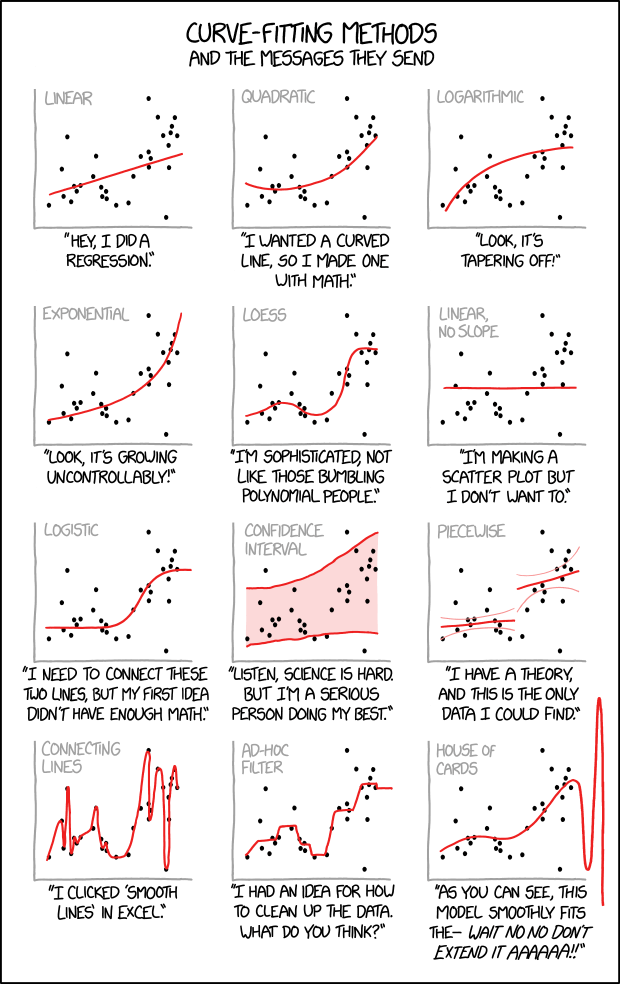
\includegraphics[width=0.49\textwidth,trim={0 16.5cm 0 0.5cm},clip]{figures/xkcd}
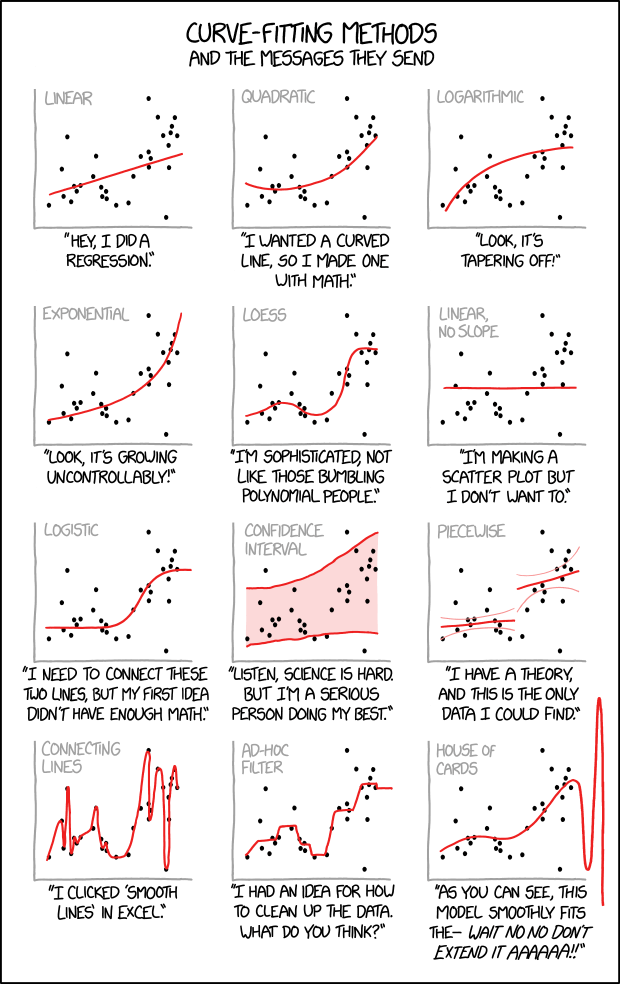
\includegraphics[width=0.49\textwidth,trim={0 0.5cm 0 16.5cm},clip]{figures/xkcd}
\end{frame}

\makebeamertitle
\mode<article>{Just in article version}


\begin{frame}
    {Complexity of Hypothesis Spaces}
    What is the trade-off between approximation error and estimation error?
    \pause
    \begin{itemize}
        \item Bigger $\sF$: better approximation but can overfit (need more samples)
        \item Smaller $\sF$: less likely to overfit but can be farther from the true function
    \end{itemize}
    \pause

    To control the ``size'' of $\sF$, we need some measure of its \hl{complexity}:
    \begin{itemize}
        \item Number of variables / features
        \item Degree of polynomial
    \end{itemize}
\end{frame}

\begin{frame}
    {General Approach to Control Complexity}
    \begin{itemize}
        \item[1.] Learn \hl{a sequence of models} varying in complexity from the training data
\[
\cf_{1}\subset\cf_{2}\subset\cf_{n}\cdots\subset\cf
\]
\pause
Example: {Polynomial Functions}
\begin{itemize}
\item $\cf=\left\{ \mbox{all polynomial functions}\right\} $
\item $\cf_{d}=\left\{ \mbox{all polynomials of degree }\le d\right\} $
\end{itemize}
\pause

        \item[2.] Select one of these models based on a score (e.g. validation error)
    \end{itemize}
\end{frame}

\begin{frame}
    {Feature Selection in Linear Regression}
    Nested sequence of hypothesis spaces:
$
\cf_{1}\subset\cf_{2}\subset\cf_{n}\cdots\subset\cf
$
    \begin{itemize}
\item $\cf=\left\{ \mbox{linear functions using all features}\right\} $
\item $\cf_{d}=\left\{ \mbox{linear functions using fewer than $d$ features}\right\} $
    \end{itemize}

    \pause
    \textbf{Best subset selection}:
    \begin{itemize}
        \item Choose the subset of features that is best according to the score (e.g. validation error)
            \begin{itemize}
                \item Example with two features:
                    Train models using $\pc{}$,
                $\pc{X_1}$,
                $\pc{X_2}$,
                $\pc{X_1, X_2}$, respectively
            \end{itemize}
        \item \al{Not an efficient search algorithm}; iterating over all subsets becomes very expensive with a large number of features 
    \end{itemize}
\end{frame}

\begin{frame}
    {Greedy Selection Methods}
    \textbf{Forward selection}:
    \begin{itemize}
        \item[1.] Start with an empty set of features $S$
        \pause
        \item[2.] For each feature $i$ not in $S$
            \begin{itemize}
                \item Learn a model using features $S\cup i$
                \item Compute score of the model: $\alpha_i$
            \end{itemize}
        \pause
        \item[3.] Find the candidate feature with the highest score: $j = \argmax_i \alpha_i$
        \pause
        \item[4.] If $\alpha_j$ improves the current best score, add feature $j$: $S\leftarrow S\cup j$ and go to step 2; return $S$ otherwise.
    \end{itemize}

    \pause
    \textbf{Backward Selection}:
    \begin{itemize}
        \item Start with all features; in each iteration, remove the worst feature
    \end{itemize}
\end{frame}

\begin{frame}
    {Feature Selection: Discussion}
    \begin{itemize}[<+->]
        \item Number of features as a measure of the complexity of a linear prediction function
        \item General approach to feature selection:
            \begin{itemize}
                \item Define a score that balances training error and complexity
                \item Find the subset of features that maximizes the score
            \end{itemize}
        \item Forward \& backward selection do not guarantee to find the best solution.
        \item Forward \& backward selection do not in general result in the same subset.
    \end{itemize}
\end{frame}

\section{$\ell_2$ and $\ell_1$ Regularization}


\begin{frame}
    {Complexity Penalty}
    An objective that balances number of features and prediction performance:

    \begin{align}
        \text{score}(S) = \text{training\_loss}(S) + \lambda |S|
    \end{align}
    \pause

    $\lambda$ balances the training loss and the number of features used:
    \begin{itemize}
        \item Adding an extra feature must be justified by at least $\lambda$ improvement in training loss
        \item Larger $\lambda$ $\rightarrow$ complex models are penalized more heavily
        % \item Criteria such as AIC and BIC use different values of $\lambda$
    \end{itemize}
\end{frame}

\begin{frame}
    {Complexity Penalty}
    \head{Goal}: Balance the complexity of the hypothesis space $\sF$ and the training loss

    \head{Complexity measure}: $\Omega:\cf\to[0,\infty)$, e.g. number of features

\pause

\begin{block}{Penalized ERM (Tikhonov regularization)}

For complexity measure $\Omega:\cf\to[0,\infty)$ and fixed $\lambda\ge0$,
\begin{align*}
\min_{f\in\cf} & \frac{1}{n}\sum_{i=1}^{n}\ell(f(x_{i}),y_{i})+\lambda\Omega(f)
\end{align*}
\end{block}

As usual, we find $\lambda$ using the validation data.

\pause

Number of features as complexity measure is hard to optimize---other measures?
\end{frame}

\begin{frame}
    {Weight Shrinkage: Intuition}
    \begin{figure}
        % 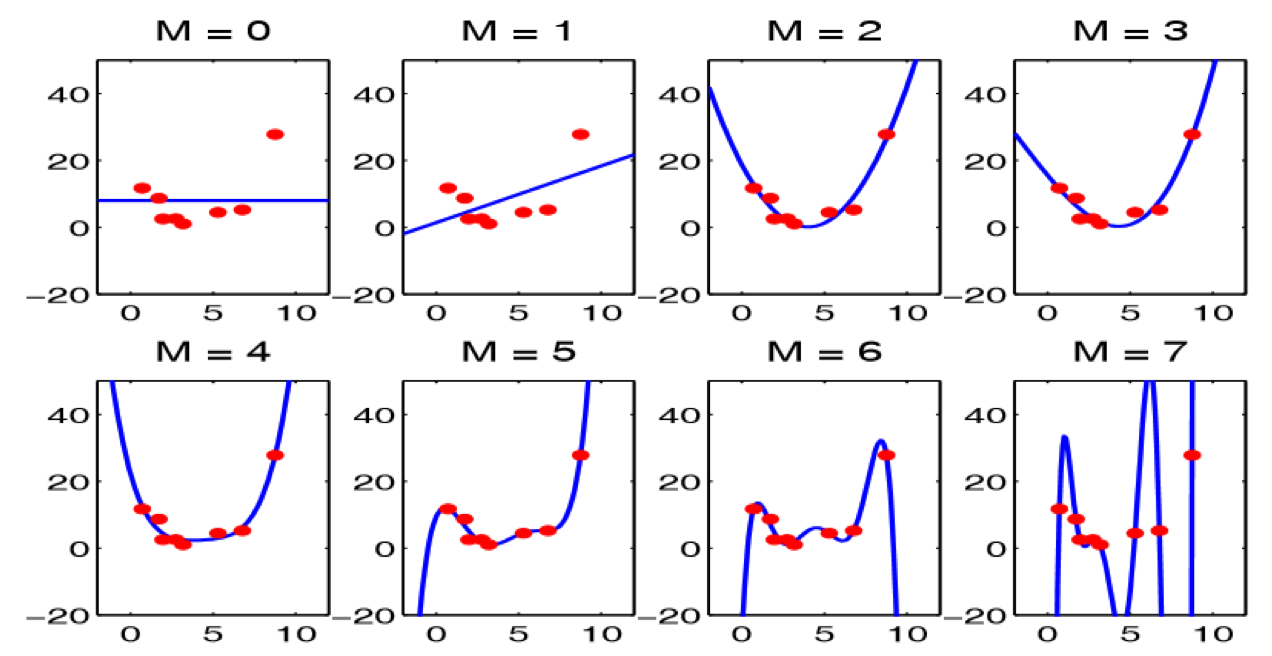
\includegraphics[height=3cm,trim={7cm 5.9cm 11cm 0},clip]{figures/poly-regression}
        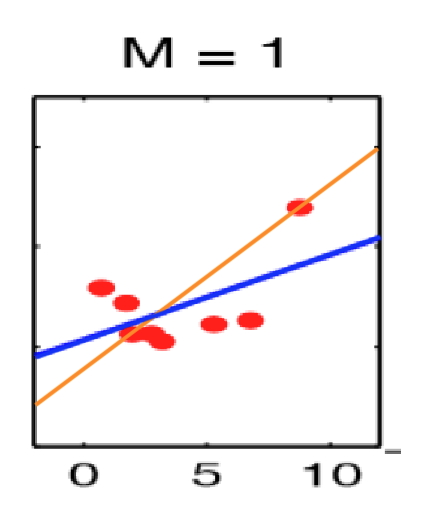
\includegraphics[height=3cm]{figures/smaller_weights}
    \end{figure}
    \begin{itemize}[<+->]
        % \item (Draw on board)
        \item Why would we prefer a regression line with \hl{smaller slope} (unless the data strongly supports a larger slope)?
        \item More conservative: small change in the input does not cause large change in the output
        \item If we push the estimated weights to be small, re-estimating them on a new dataset wouldn't cause the prediction function to change dramatically (\hl{less sensitive to noise in data})
        % \item Bayesian intuition: our ``prior'' intuition is that weights are small and centered at 0. Pull the regression weights towards a prior centered at 0
    \end{itemize}
\end{frame}

\begin{frame}
    {Weight Shrinkage: Polynomial Regression}
    \begin{figure}
        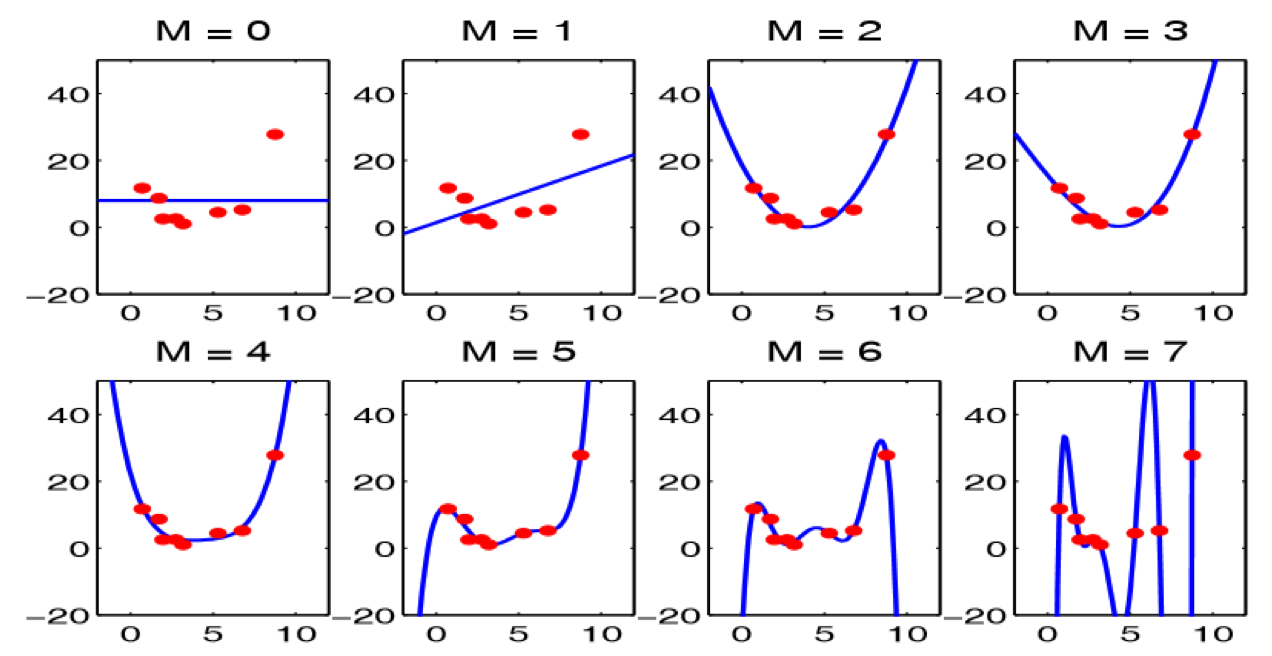
\includegraphics[height=4.5cm]{figures/poly-regression}
    \end{figure}
    \begin{itemize}
    \vspace{-0.5cm}
    \item Large weights are needed to make the curve wiggle sufficiently to overfit the data
    \item $\hat{y} = 0.001x^7 + 0.003x^3 + 1$ less likely to overfit than $\hat{y} = 1000x^7 + 500x^3 + 1$
    \end{itemize}
    \small{(Adapated from Mark Schmidt's slide)}
\end{frame}

\begin{frame}
    {Linear Regression with $\ell_2$ Regularization}
\begin{itemize}
\item We have a linear model
\[
\cf=\left\{ f:\reals^{d}\to\reals\mid f(x)=w^{T}x\mbox{ for }w\in\reals^{d}\right\} 
\]
\item Square loss: $\loss(\hat{y},y)=(y-\hat{y})^{2}$
\item Training data $\cd_{n}=\left((x_{1},y_{1}),\ldots,(x_{n},y_{n})\right)$
\pause
\item Linear least squares regression is ERM for square loss over $\cf$:
\[
\hat{w}=\argmin_{w\in\reals^{d}}\frac{1}{n}\sum_{i=1}^{n}( w^{T}x_{i}-y_{i}) ^{2}
\]
\item This often overfits, especially when $d$ is large compared to $n$ (e.g. in NLP one can have 
1M features for 10K documents).
\end{itemize}
\end{frame}

\begin{frame}
    {Linear Regression with L2 Regularization}
    \hl{Penalizes large weights}:
\[
\hat{w}=\argmin_{w\in\reals^{d}}\frac{1}{n}\sum_{i=1}^{n}\left\{ w^{T}x_{i}-y_{i}\right\} ^{2}+
    {\color{blue}\lambda\|w\|_{2}^{2}},
\]
where $\|w\|_{2}^{2}=w_{1}^{2}+\cdots+w_{d}^{2}$ is the square of
the $\ell_{2}$-norm.

\medskip
\begin{itemize}
    \item Also known as \textbf{ridge regression}.
        \pause
    \item Equivalent to linear least square regression when $\lambda=0$.
    \pause
    \item $\ell_2$ regularization can be used for other models too (e.g. neural networks).
\end{itemize}
\end{frame}

\begin{frame}{$\ell_{2}$ regularization reduces sensitivity to changes in input}
\begin{itemize}
\item $\hat{f}(x)=\hat{w}^{T}x$ is \textbf{Lipschitz continuous
}with Lipschitz constant $L=\|\hat{w}\|_{2}$: when moving from $x$ to $x+h$, $\hat{f}$ changes
no more than $L\|h\|$. 
\pause

\item $\ell_{2}$ regularization controls the maximum rate of change
of $\hat{f}$.
\pause

\item Proof:
\begin{eqnarray*}
\left|\hat{f}(x+h)-\hat{f}(x)\right| & = & |\hat{w}^{T}\left(x+h\right)-\hat{w}^{T}x|=\left|\hat{w}^{T}h\right|\\
 & \le & \|\hat{w}\|_{2}\|h\|_{2}\quad\text{(Cauchy-Schwarz inequality)}
\end{eqnarray*}

\pause
\item Other norms also provide a bound on $L$ due to the equivalence of norms: $\exists C>0 \text{ s.t. } \|\hat{w}\|_2 \le C\|\hat{w}\|_p$
\end{itemize}
\end{frame}

\begin{frame}
    {Linear Regression vs. Ridge Regression}
    \head{Objective}:\\
    \begin{itemize}
        \setlength\itemsep{1ex}
        \item Linear: $L(w) = \frac{1}{2}\|Xw - y\|_2^2$
        \item Ridge: $L(w) = \frac{1}{2}\|Xw - y\|_2^2 + {\color{blue}\frac{\lambda}{2}{\|w\|_2^2}}$
    \end{itemize}
    \pause

    \head{Gradient}:\\
    \begin{itemize}
        \setlength\itemsep{1ex}
        \item Linear: $\nabla L(w) = X^T(Xw - y)$
        \item Ridge: $\nabla L(w) = X^T(Xw - y) + {\color{blue}\lambda w}$
            \begin{itemize}
                \item Also known as \textbf{weight decay} in neural networks
            \end{itemize}
    \end{itemize}
    \pause

    \head{Closed-form solution}:\\
    \begin{itemize}
        \setlength\itemsep{1ex}
        \item Linear: $X^TXw = X^Ty$
        \item Ridge: $(X^TX + {\color{blue}\lambda I})w = X^Ty$
            \begin{itemize}
                \item $(X^TX + {\color{blue}\lambda I})$ is always invertible
            \end{itemize}
    \end{itemize}
\end{frame}

\begin{frame}{Ridge Regression: Regularization Path}
    %\textbf{Regulariztion path} shows how the weights vary as we change the regularization strength

% There are five predictors: 
% - annual police funding in dollars per resident (funding)
% - percent of people 25 years and older with four years of high school (hs)
% - percent of 16- to 19-year olds not in high school and not high school graduates (not-hs)
% - percent of 18- to 24-year olds in college (college)
% - percent of people 25 years and older with at least four years of college. (college4)
% This small example is for illustration only, but helps to demonstrate the nature of the
% lasso solutions. Typically the lasso is most useful for much larger problems,
% including “wide” data for which p >> N.

\let\thefootnote\relax\footnotetext{\tiny{Modified from Hastie, Tibshirani, and Wainwright's \emph{Statistical Learning with Sparsity}, Fig 2.1. About predicting crime in 50 US cities.}}
\begin{center}
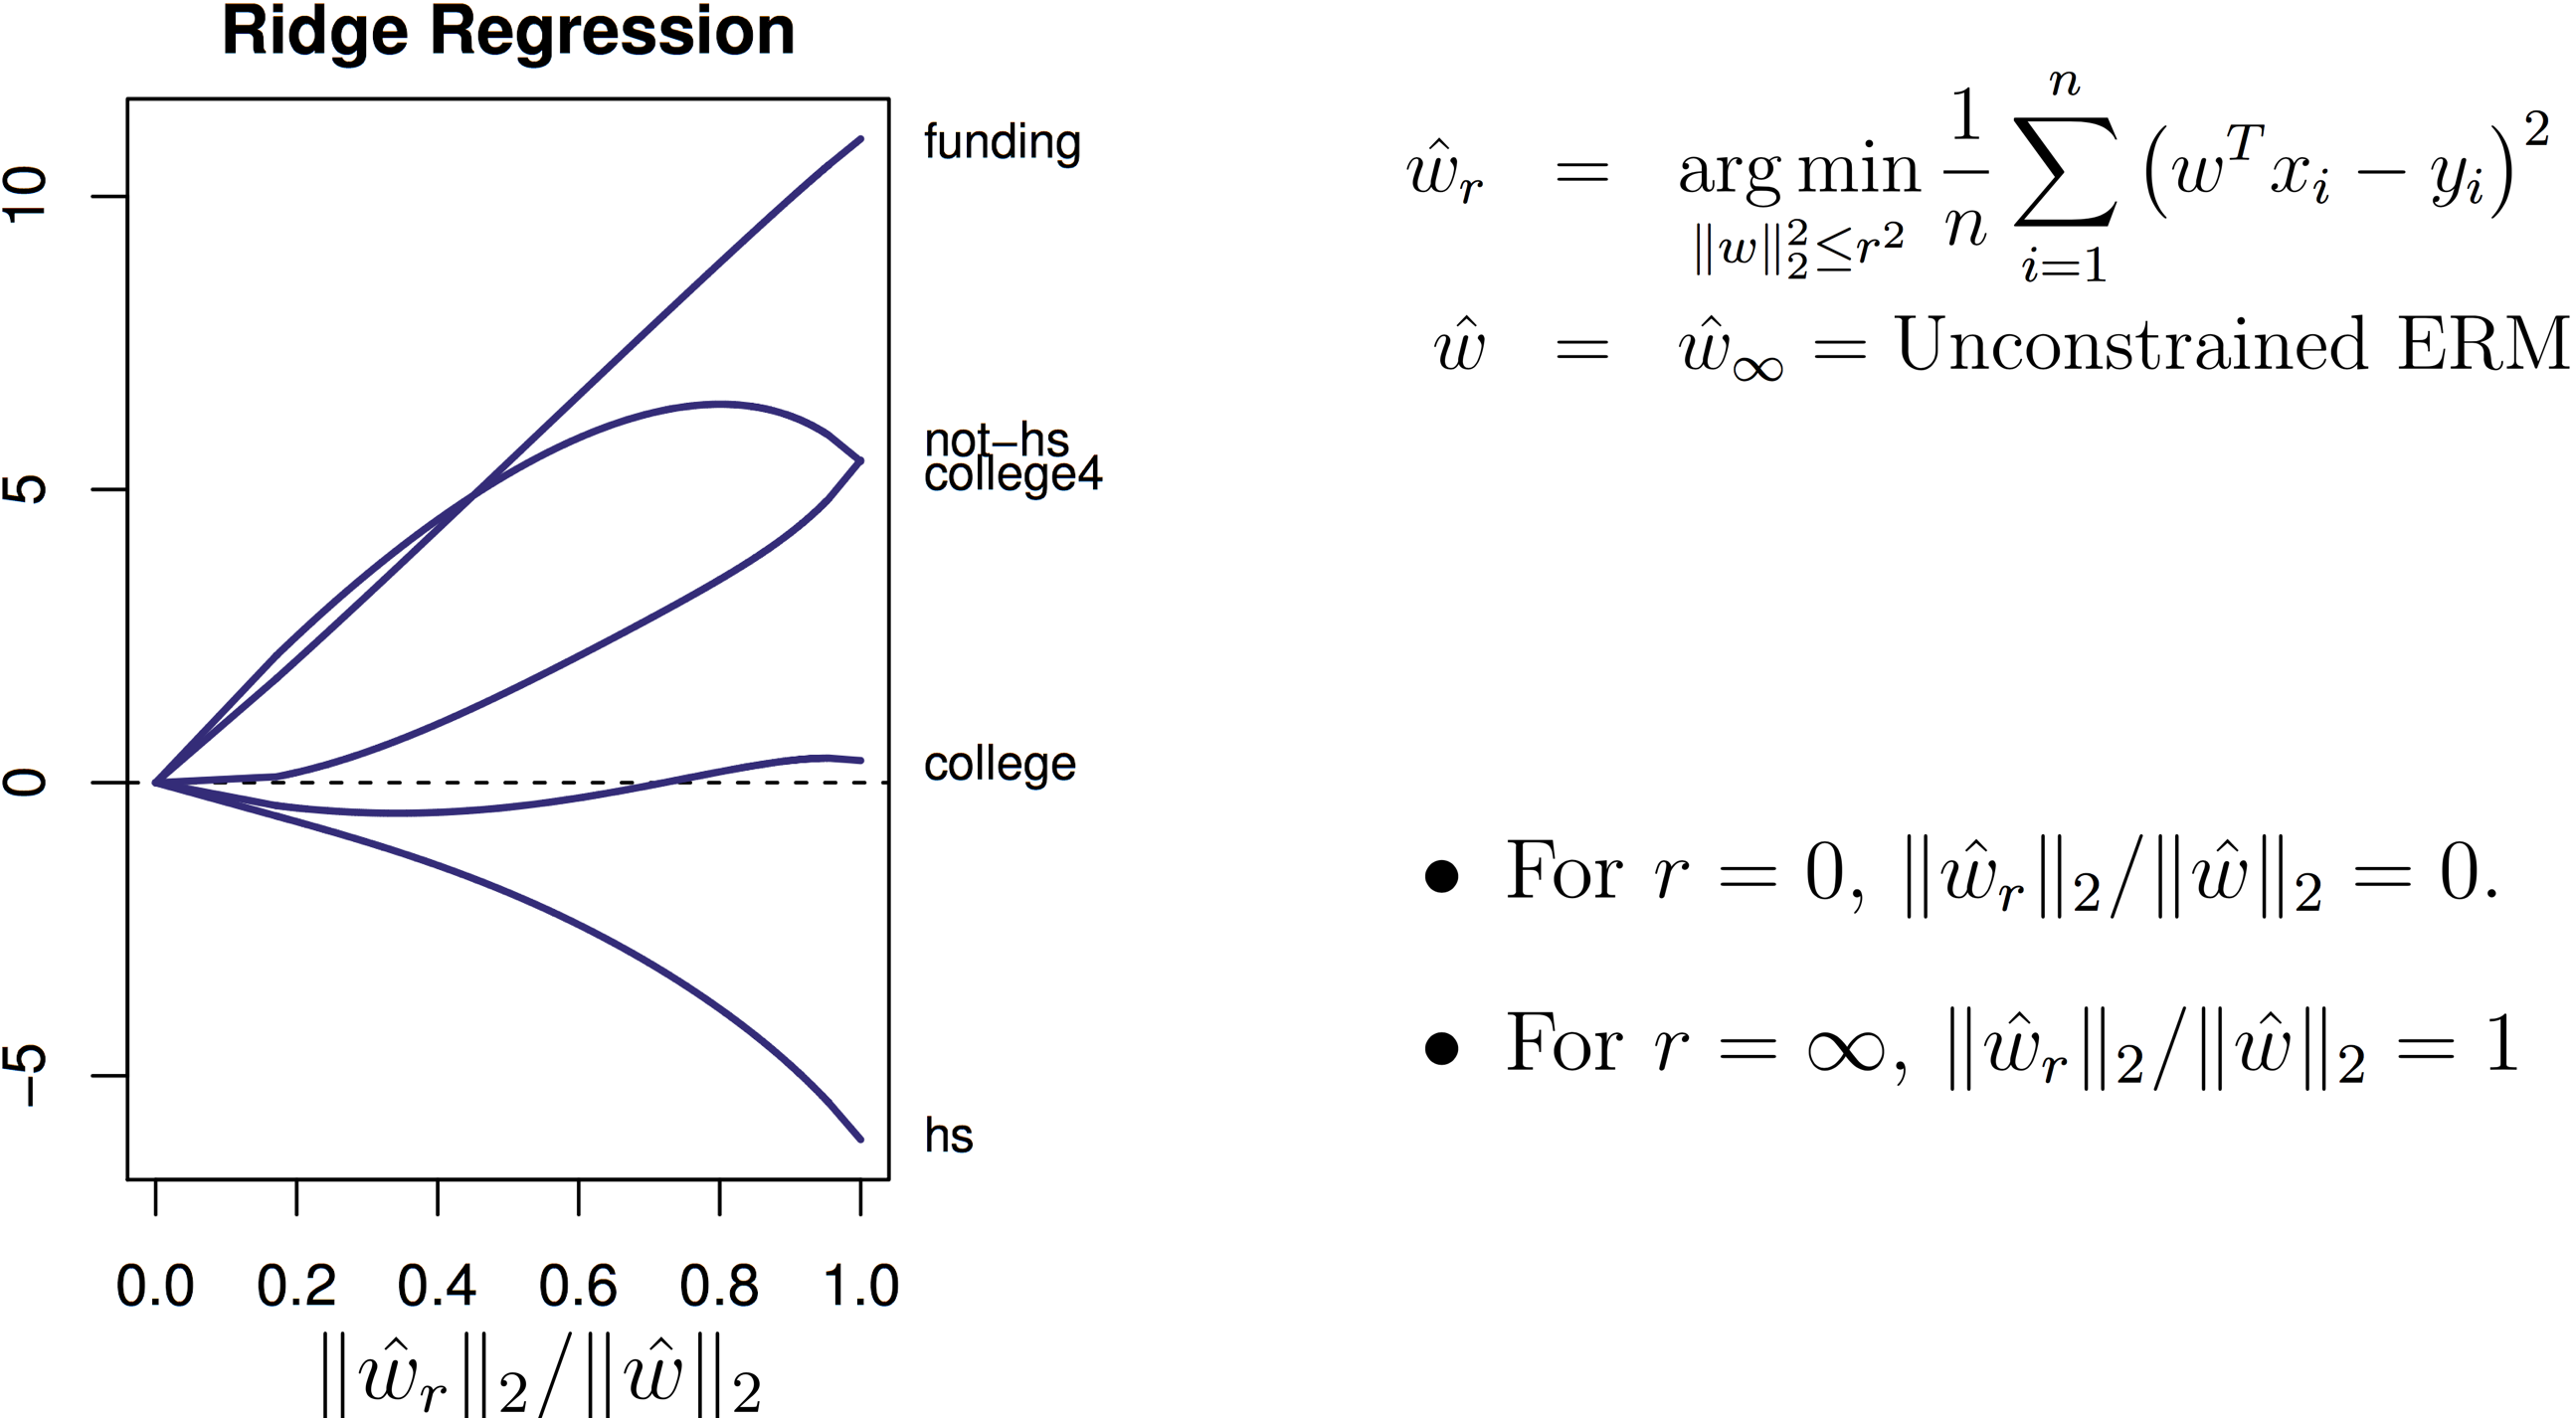
\includegraphics[height=0.7\textheight]{figures/ridge-regularization-HTW-Fig21-LATEX.png} 
\par\end{center}
\end{frame}

\begin{frame}{Lasso Regression}
    Penalize the $\ell_1$ norm of the weights:
\begin{block}{Lasso Regression (Tikhonov Form, soft penalty)}
\[
\hat{w}=\argmin_{w\in\reals^{d}}\frac{1}{n}\sum_{i=1}^{n}\left\{ w^{T}x_{i}-y_{i}\right\} ^{2}+\lambda\|w\|_{1},
\]
where $\|w\|_{1}=\left|w_{1}\right|+\cdots+\left|w_{d}\right|$ is
the $\ell_{1}$-norm.
\end{block}

        (``Least Absolute Shrinkage and Selection Operator'')
\end{frame}

\begin{frame}{Ridge vs. Lasso: Regularization Paths}
Lasso yields sparse weights:

\let\thefootnote\relax\footnotetext{\tiny{Modified from Hastie, Tibshirani, and Wainwright's \emph{Statistical Learning with Sparsity}, Fig 2.1. About predicting crime in 50 US cities.}}
\begin{center}
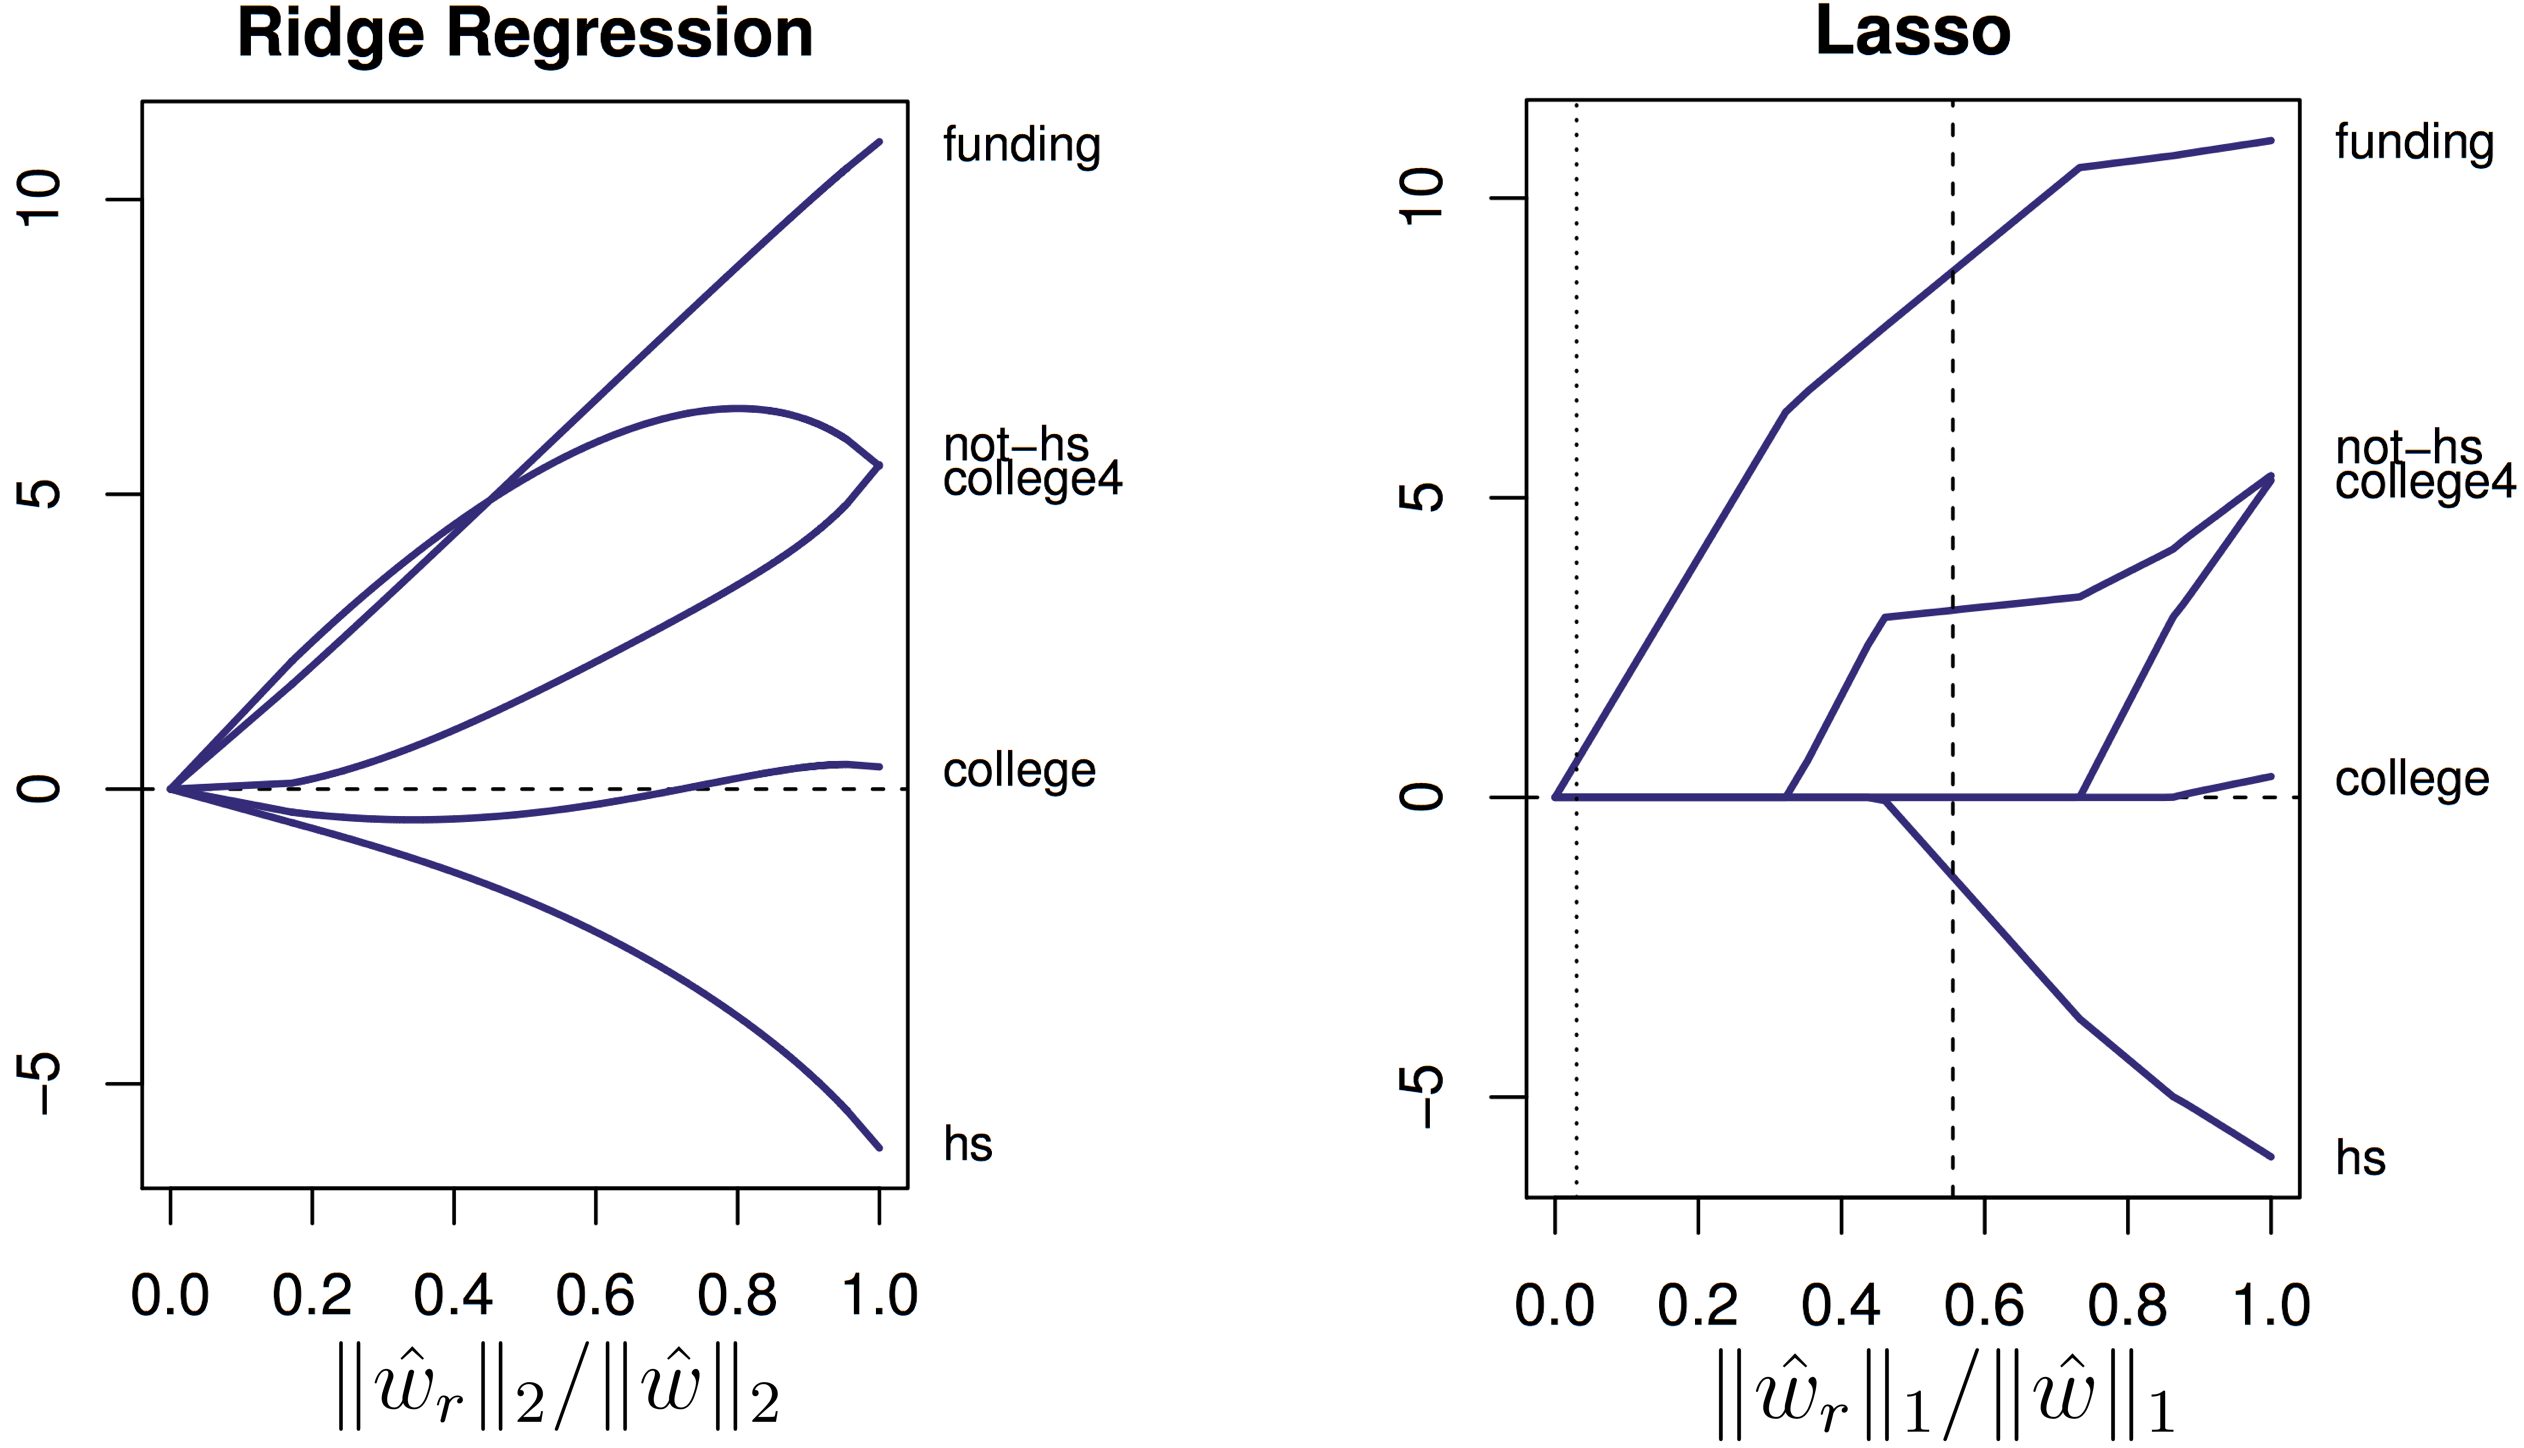
\includegraphics[height=0.7\textheight]{figures/lasso-ridge-paths-side-by-side}
\par\end{center}
\end{frame}

\begin{frame}{The Benefits of Sparsity}

The coefficient for a feature is $0$ $\implies$ the feature is not needed for prediction. Why is that useful?

\pause
    \begin{itemize}[<+->]
\item Faster to compute the features; cheaper to measure or annotate them

\item Less memory to store features (deployment on a mobile device)

\item Interpretability: identifies the important features

\item Prediction function may generalize better (model is less complex)

% \item Feature-selection step for training a slower non-linear model
\end{itemize}
\end{frame}

\section{Why does $\ell_1$ Regularization Lead to Sparsity?}
\begin{frame}{Regularization as Constrained Empirical Risk Minimization}
\begin{block}{Constrained ERM (Ivanov regularization)}
For complexity measure $\Omega:\cf\to[0,\infty)$ and fixed $r\ge0$,
\begin{align*}
\min_{f\in\cf}\; & \frac{1}{n}\sum_{i=1}^{n}\ell(f(x_{i}),y_{i})\\
\mbox{s.t.}\; & \Omega(f)\le r
\end{align*}
\end{block}

\begin{block}{Lasso Regression (Ivanov Form, hard constraint)}
The lasso regression solution for complexity parameter $r\ge0$ is
\[
\hat{w}=\argmin_{\|w\|_{1}\le r}\frac{1}{n}\sum_{i=1}^{n}\left\{ w^{T}x_{i}-y_{i}\right\} ^{2}.
\]
\end{block}
    $r$ has the same role as $\lambda$ in penalized ERM (Tikhonov).
\end{frame}

\begin{frame}{Ivanov vs. Tikhonov Regularization}
\begin{itemize}
\item Let $L:\cf\to\reals$ be any performance measure of $f$
\begin{itemize}
\item e.g. $L(f)$ could be the empirical risk of $f$
\end{itemize}
\pause

\item For many $L$ and $\Omega$, Ivanov and Tikhonov are equivalent:
\begin{itemize}
\item Any solution $f^{*}$ we can get from Ivanov, we can also get from
Tikhonov.
\item Any solution $f^{*}$ we can get from Tikhonov, we can also get from
Ivanov.
\end{itemize}
\pause
\item The conditions for this equivalence can be derived from Lagrangian duality theory.
\pause
\item In practice, both approaches are effective: we will use whichever one is more convenient for training or analysis. 
\end{itemize}
\end{frame}

%\begin{frame}{Ivanov vs Tikhonov Regularization (Details) }
%Ivanov and Tikhonov regularization are equivalent if:
%\begin{enumerate}
%\item For any choice of $r>0$, any Ivanov solution
%\[
%\minimizer{f_{r}}\in\argmin_{\substack{f\in\cf}
%}L(f)\mbox{ s.t. }\Omega(f)\le r
%\]
%is also a Tikhonov solution for some $\lambda>0$. That is, $\exists\lambda>0$
%such that
%\[
%\minimizer{f_{r}}\in\argmin_{f\in\cf}L(f)+\lambda\Omega(f).
%\]


%\item Conversely, for any choice of $\lambda>0$, any Tikhonov solution:
%\[
%\minimizer{f_{\lambda}}\in\argmin_{f\in\cf}L(f)+\lambda\Omega(f)
%\]
%is also an Ivanov solution for some $r>0$. That is, $\exists r>0$
%such that
%\[
%\minimizer{f_{\lambda}}\in\argmin_{\substack{f\in\cf}
%}L(f)\mbox{ s.t. }\Omega(f)\le r
%\]
%\end{enumerate}
%\end{frame}

\begin{frame}{The $\ell_{1}$ and $\ell_{2}$ Norm Constraints}
\begin{itemize}
\item Let's consider $\cf=\left\{ f(x)=w_{1}x_{1}+w_{2}x_{2}\right\} $
space)

\item We can represent each function in $\cf$ as a point $(w_{1},w_{2})\in\reals^{2} .$

\item Where in $\reals^{2}$ are the functions that satisfy the Ivanov regularization constraint for $\ell_{1}$ and $\ell_{2}$?
\end{itemize}

\pause
\begin{columns}[t]

\column{.3\textwidth}
\begin{itemize}
\item $\ell_{2}$ contour: $w_{1}^{2}+w_{2}^{2}=r$
\end{itemize}
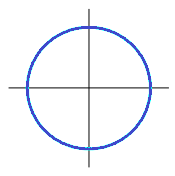
\includegraphics[height=0.25\textheight]{figures/l2Contour}


\column{.3\textwidth}
\begin{itemize}
\item $\ell_{1}$ contour: $\left|w_{1}\right|+\left|w_{2}\right|=r$ 
\end{itemize}
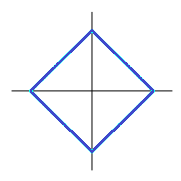
\includegraphics[height=0.25\textheight]{figures/l1Countour}
\end{columns}
\pause
    \begin{itemize}
    \item Where are the sparse solutions?
    \end{itemize}
\end{frame}

\begin{frame}{Visualizing Regularization}

\begin{itemize}
\item $\minimizer{f_{r}}=\argmin_{w\in\reals^{2}}\sum_{i=1}^{n}\left(w^{T}x_{i}-y_{i}\right)^{2}\,\text{subject to }w_{1}^{2}+w_{2}^{2}\le r$
\end{itemize}
\begin{center}
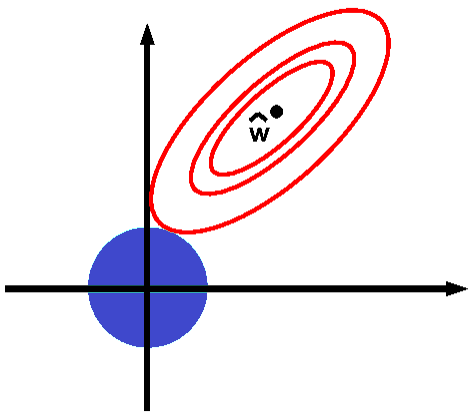
\includegraphics[height=0.4\textheight]{figures/l2LossConstraintPic}\vspace{-0.3cm}
\par\end{center}
\begin{itemize}
        \setlength\itemsep{1ex}
\item Blue region: Area satisfying complexity constraint: $w_{1}^{2}+w_{2}^{2}\le r$
\item Red lines: contours of the empirical risk $\hat{R}_{n}(w)=\sum_{i=1}^{n}\left(w^{T}x_{i}-y_{i}\right)^{2}$. 
\end{itemize}
\let\thefootnote\relax\footnotetext{\tiny{KPM Fig. 13.3}}
\end{frame}

\begin{frame}{Why Does $\ell_{1}$ Regularization Encourage Sparse Solutions?}
\let\thefootnote\relax\footnotetext{\tiny{KPM Fig. 13.3}}
\begin{itemize}
\item $\minimizer{f_{r}}=\argmin_{w\in\reals^{2}}\frac{1}{n}\sum_{i=1}^{n}\left(w^{T}x_{i}-y_{i}\right)^{2}\,\text{subject to}\left|w_{1}\right|+\left|w_{2}\right|\le r$
\end{itemize}
\begin{center}
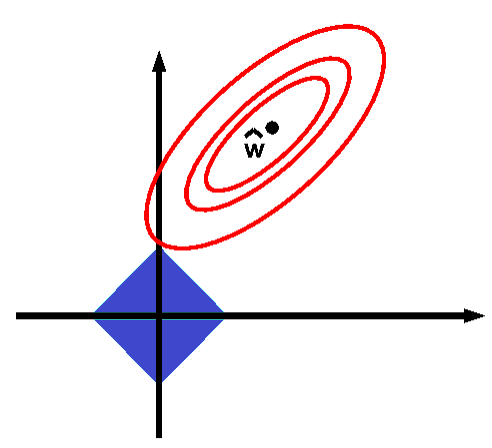
\includegraphics[height=0.4\textheight]{figures/l1LossConstraintPic}\vspace{-0.3cm}
\par\end{center}
\begin{itemize}
        \setlength\itemsep{1ex}
\item Blue region: Area satisfying complexity constraint: $\left|w_{1}\right|+\left|w_{2}\right|\le r$
\item Red lines: contours of the empirical risk $\hat{R}_{n}(w)=\sum_{i=1}^{n}\left(w^{T}x_{i}-y_{i}\right)^{2}$. 
\item $\ell_1$ solution tends to touch the \hl{corners}.
\end{itemize}
\end{frame}

\begin{frame}
    {Why Does $\ell_1$ Regularization Encourage Sparse Solutions?}
    \head{Geometric intuition}: Projection onto diamond encourages solutions at corners.
    \begin{itemize}
        \item $\hat{w}$ in red/green regions are closest to corners in the $\ell_1$ ``ball''.
    \end{itemize}

\let\thefootnote\relax\footnotetext{\tiny{Fig from \href{https://arxiv.org/abs/1411.3230}{Mairal et al.'s Sparse Modeling for Image and Vision Processing} Fig 1.6}}
\begin{center}
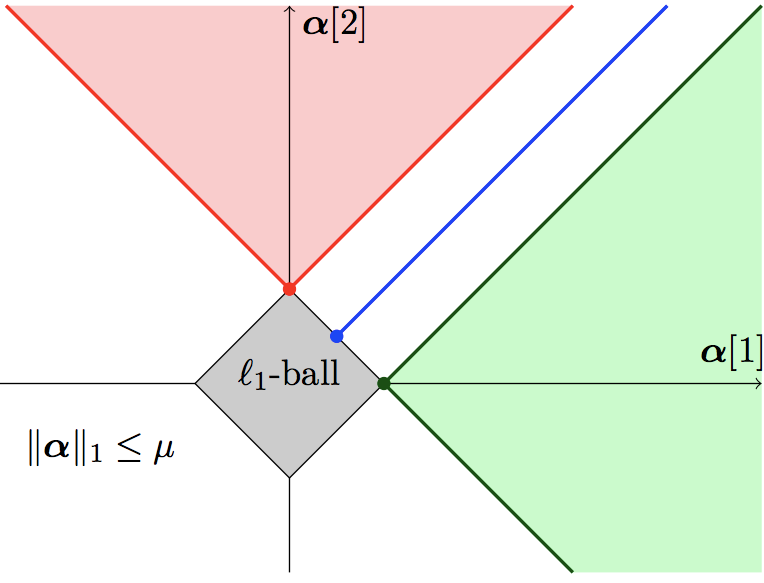
\includegraphics[height=0.5\textheight]{figures/projections-to-L1Ball}\vspace{-0.3cm}
\par\end{center}
\end{frame}

\begin{frame}
    {Why Does $\ell_1$ Regularization Encourage Sparse Solutions?}
    \head{Geometric intuition}: Projection onto $\ell_2$ sphere favors all directions equally.

\let\thefootnote\relax\footnotetext{\tiny{Fig from \href{https://arxiv.org/abs/1411.3230}{Mairal et al.'s Sparse Modeling for Image and Vision Processing} Fig 1.6}}
\begin{center}
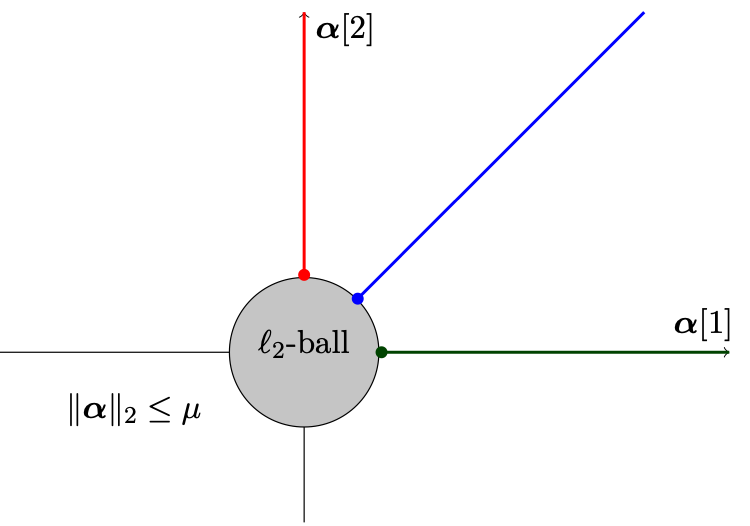
\includegraphics[height=0.5\textheight]{figures/projections-to-L2Ball}\vspace{-0.3cm}
\par\end{center}
\end{frame}

\begin{frame}{Why does $\ell_2$ Encourage Sparsity? Optimization Perspective}
    For $\ell_2$ regularization,
    \begin{itemize}
        \item As $w_i$ becomes smaller, there is less and less penalty 
            \begin{itemize}
                \item What is the $\ell_2$ penalty for $w_i=0.0001$?
            \end{itemize}
        \item The gradient---which determines the pace of optimization---decreases as $w_i$ approaches zero 
        \item Less incentive to make a small weight equal to exactly zero
    \end{itemize}
    \pause

    For $\ell_1$ regularization,
    \begin{itemize}
        \item The gradient stays the same as the weights approach zero
        \item This pushes the weights to be exactly zero even if they are already small
    \end{itemize}

\end{frame}

\begin{frame}{$\left(\ell_{q}\right)$ Regularization}
\begin{itemize}
\item We can generalize to $\ell_{q}$ : $\left(\|w\|_{q}\right)^{q}=\left|w_{1}\right|^{q}+\left|w_{2}\right|^{q}$.
    \pause
\end{itemize}
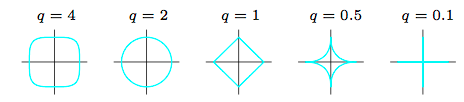
\includegraphics[width=0.8\columnwidth]{figures/LqNormContours}

\begin{itemize}
\pause
\item Note: $\|w\|_{q}$ is only a norm if $q\ge1$, but not for $q\in\left(0,1\right)$
\pause
\item When $q<1$, the $\ell_q$ constraint is non-convex, so it is hard to optimize; lasso is good enough in practice
\pause
\item $\ell_0$ ($\|w\|_0$) is defined as the number of non-zero weights, i.e. subset selection
\end{itemize}
\end{frame}

\section{Minimizing the lasso objective}

\begin{frame}{Minimizing the lasso objective}
\begin{itemize}
    \item The ridge regression objective is differentiable (and there is a closed form solution)
\item Lasso objective function:
\[
\min_{w\in\reals^{d}}\sum_{i=1}^{n}\left(w^{T}x_{i}-y_{i}\right)^{2}+\lambda\|w\|_{1}
\]
\item $\|w\|_{1}=\left|w_{1}\right|+\ldots+\left|w_{d}\right|$ is not differentiable!
\pause
\item We will briefly review three approaches for finding the minimum:
    \begin{itemize}
        \item Quadratic programming
        \item Projected SGD
        \item Coordinate descent
    \end{itemize}
\end{itemize}
\end{frame}

\begin{frame}{ Rewriting the Absolute Value}
\begin{itemize}
\item Consider any number $a\in\reals$.
\item Let the \textbf{positive part} of $a$ be
\[
a^{+}=a\ind{a\ge0}.
\]


\item Let the \textbf{negative part} of $a$ be
\[
a^{-}=-a\ind{a\le0}.
\]

\pause
\item Is it always the case that $a^{+}\ge0$ and $a^{-}\ge0$?

\pause
\item How do you write $a$ in terms of $a^{+}$ and $a^{-}$?

\pause
\item How do you write $\left|a\right|$ in terms of $a^{+}$ and $a^{-}$?
\end{itemize}
\end{frame}

\begin{frame}{The Lasso as a Quadratic Program}

Substituting $w=w^{+}-w^{-}$ and $\left|w\right|=w^{+}+w^{-}$
results in an \hl{equivalent} problem:
\begin{align*}
\min_{w^{+},w^{-}}\quad & \sum_{i=1}^{n}\left(\left(w^{+}-w^{-}\right)^{T}x_{i}-y_{i}\right)^{2}+\lambda1^{T}\left(w^{+}+w^{-}\right)\\
\mbox{subject to}\quad & w_{i}^{+}\ge0\mbox{ for all }i\text{\quad and \quad}w_{i}^{-}\ge0\mbox{ for all }i,
\end{align*}


\begin{itemize}
\item This objective is \textbf{differentiable} (in fact, \textbf{convex and
quadratic})
\item How many variables does the new objective have?
\item This is a \textbf{quadratic program}: a convex quadratic objective with
linear constraints.
\item Quadratic programming is a very well understood problem; we can plug this into a generic QP solver.
\end{itemize}
\end{frame}

\begin{frame}{Are we missing some constraints?}

We have claimed that the following objective is equivalent to the lasso problem:
\begin{align*}
\min_{w^{+},w^{-}}\quad & \sum_{i=1}^{n}\left(\left(w^{+}-w^{-}\right)^{T}x_{i}-y_{i}\right)^{2}+\lambda1^{T}\left(w^{+}+w^{-}\right)\\
\mbox{subject to}\quad & w_{i}^{+}\ge0\mbox{ for all }i\text{\qquad}w_{i}^{-}\ge0\mbox{ for all }i,
\end{align*}


\begin{itemize}
\item When we plug this optimization problem into a QP solver,
\begin{itemize}
\item it just sees $2d$ variables and $2d$ constraints.
\item \al{Doesn't know we want $w_{i}^{+}$ and $w_{i}^{-}$ to be positive
    and negative parts of $w_{i}$}.
\end{itemize}
\item Turns out that these constraints will be satisfied anyway!
\item To make it clear that the solver isn't aware of the constraints of $w_{i}^{+}$ and $w_{i}^{-}$, let's denote them $a_i$ and $b_{i}$
\end{itemize}
\end{frame}

\begin{frame}{The Lasso as a Quadratic Program}

    (Trivially) reformulating the lasso problem:
\begin{align*}
\min_{w}\;\min_{a,b}\quad & \sum_{i=1}^{n}\left(\left(a-b\right)^{T}x_{i}-y_{i}\right)^{2}+\lambda1^{T}\left(a+b\right)\\
\mbox{subject to}\quad & a_{i}\ge0\mbox{ for all }i\text{\qquad}b_{i}\ge0\mbox{ for all }i,\\
 & a-b=w\\
 & a+b=|w|
\end{align*}

\pause

    \head{Claim}: Don't need the constraint $a+b=|w|$. 

    \head{Exercise}: Prove by showing that the optimal solutions $a^*$ and $b^*$ satisfies $\min(a^*, b^*)=0$, hence $a^*+b^*=|w|$.
\end{frame}

\begin{frame}{The Lasso as a Quadratic Program}

\begin{align*}
\min_{w}\;\min_{a,b}\quad & \sum_{i=1}^{n}\left(\left(a-b\right)^{T}x_{i}-y_{i}\right)^{2}+\lambda1^{T}\left(a+b\right)\\
\mbox{subject to}\quad & a_{i}\ge0\mbox{ for all }i\text{\qquad}b_{i}\ge0\mbox{ for all }i,\\
 & a-b=w
\end{align*}

    \head{Claim}: Can remove $\min_{w}$ and the constraint $a-b=w$. 

    \head{Exercise}: Prove by switching the order of the minimization.
\end{frame}

\begin{frame}{Projected SGD}
\begin{itemize}
    \item Now that we have a differentiable objective, we could also use gradient descent
\item But how do we handle the \hl{constraints}?
\end{itemize}
\begin{align*}
\min_{w^{+},w^{-}\in\reals^{d}} & \sum_{i=1}^{n}\left(\left(w^{+}-w^{-}\right)^{T}x_{i}-y_{i}\right)^{2}+\lambda1^{T}\left(w^{+}+w^{-}\right)\\
\mbox{subject to } & w_{i}^{+}\ge0\mbox{ for all }i\\
 & w_{i}^{-}\ge0\mbox{ for all }i
\end{align*}

\begin{itemize}
\item Projected SGD is just like SGD, but after each step
\begin{itemize}
\item We project $w^{+}$ and $w^{-}$ into the constraint set.
\item In other words, if any component of $w^{+}$ or $w^{-}$ becomes negative,
we set it back to 0.
\end{itemize}
\end{itemize}
\end{frame}

\begin{frame}{Coordinate Descent Method}

\head{Goal}: Minimize $L(w)=L(w_{1},\ldots,w_{d})$ over $w=\left(w_{1},\ldots,w_{d}\right)\in\reals^{d}$.

\pause
    \begin{itemize}
        \item In gradient descent or SGD, 
    each step potentially changes \hl{all entries} of $w$.

\pause

\item In \textbf{coordinate descent}, 
    each step adjusts only a \hl{single coordinate} $w_{i}$.
\end{itemize}

\[
w_{i}^{\mbox{new}}=\argmin_{w_{i}}L(w_{1},\ldots,w_{i-1},\mathbf{w_{i}},w_{i+1},\ldots,w_{d})
\]

\begin{itemize}
\item Solving the argmin for a particular coordinate may itself be an iterative process. 
\item Coordinate descent is an effective method when 
    it's easy (or easier) to minimize w.r.t. one coordinate at a time 
\end{itemize}
\end{frame}


\begin{frame}{Coordinate Descent Method}

    \begin{block}{}
\textbf{Goal: }Minimize $L(w)=L(w_{1},\ldots w_{d})$ over $w=\left(w_{1},\ldots,w_{d}\right)\in\reals^{d}$.
\begin{itemize}
\item \textbf{Initialize} $w^{(0)}=0$
\item \textbf{while} not converged:
\begin{itemize}
\item Choose a coordinate $j\in\left\{ 1,\ldots,d\right\} $
\item $w_{j}^{\mbox{new}}\gets\argmin_{w_{j}}L(w_{1}^{(t)},\ldots,w_{j-1}^{(t)},\mathbf{w_{j}},w_{j+1}^{(t)},\ldots,w_{d}^{(t)})$
\item $w_{j}^{(t+1)}\gets w_{j}^{\mbox{new}}$ and $w^{(t+1)}\gets w^{(t)}$
\item $t\gets t+1$
\end{itemize}
\end{itemize}
    \end{block}

\begin{itemize}
\item Random coordinate choice $\implies$\textbf{stochastic coordinate
descent}
\item Cyclic coordinate choice $\implies$ \textbf{cyclic coordinate descent}
\end{itemize}
\end{frame}

\begin{frame}{Coordinate Descent Method for Lasso}

The lasso objective coordinate minimization has a closed form! If

\[
\hat{w}_{j}=\argmin_{w_{j}\in\reals}\sum_{i=1}^{n}\left(w^{T}x_{i}-y_{i}\right)^{2}+\lambda\left|w\right|_{1}
\]


Then
\[
\hat{w}_{j}=\begin{cases}
(c_{j}+\lambda)/a_{j} & \mbox{if }c_{j}<-\lambda\\
0 & \mbox{if }c_{j}\in[-\lambda,\lambda]\\
(c_{j}-\lambda)/a_{j} & \mbox{if }c_{j}>\lambda
\end{cases}
\]

\begin{align*}
a_{j} & =2\sum_{i=1}^{n}x_{i,j}^{2}\qquad & c_{j} & =2\sum_{i=1}^{n}x_{i,j}(y_{i}-w_{-j}^{T}x_{i,-j})
\end{align*}
where $w_{-j}$ is $w$ without the $j$-th component, and $x_{i,-j}$ is $x_i$ without the $j$-th component.
\end{frame}

\begin{frame}
    {Coordinate Descent in General}
    \begin{itemize}[<+->]
        \item In general, coordinate descent is not competitive with gradient descent: its convergence rate is slower and the iteration cost is similar
        \item But it works very well for certain problems
        \item Very simple and easy to implement
        \item Example applications: lasso regression, SVMs
    \end{itemize}
\end{frame}

\end{document}
